%; whizzy chapter
% -initex iniptex -latex platex -format platex -bibtex jbibtex -fmt fmt
% 以上 whizzytex を使用する場合の設定。

%     Tokyo Debian Meeting resources
%     Copyright (C) 2006 Junichi Uekawa

%     This program is free software; you can redistribute it and/or modify
%     it under the terms of the GNU General Public License as published by
%     the Free Software Foundation; either version 2 of the License, or
%     (at your option) any later version.

%     This program is distributed in the hope that it will be useful,
%     but WITHOUT ANY WARRANTY; without even the implied warranty of
%     MERCHANTABILITY or FITNESS FOR A PARTICULAR PURPOSE.  See the
%     GNU General Public License for more details.

%     You should have received a copy of the GNU General Public License
%     along with this program; if not, write to the Free Software
%     Foundation, Inc., 51 Franklin St, Fifth Floor, Boston, MA  02110-1301 USA

%   Pdf作成手順
% dvipdfmx debianmeetingresume200606.dvi
%  preview (shell-command (concat "xpdf " (replace-regexp-in-string "tex$" "pdf"(buffer-file-name)) "&"))
% 画像ファイルを処理するためにはebbを利用してboundingboxを作成。
%(shell-command "cd image200606; ebb *.png")

%%ここからヘッダ開始。

\documentclass[mingoth,a4paper]{jsarticle}
\usepackage[dvipdfmx]{graphicx}
\usepackage{fancybox}
\usepackage{longtable}
\usepackage{ascmac}	% 囲み (screen,itembox)
\usepackage{fancyvrb}   % 囲み Verbatim のために必要
\usepackage[dvipdfmx]{hyperref}
\usepackage{url}
\usepackage[dvipdfmx]{color}

%http://www.naney.org/diki/dk/hyperref.html
%日本語EUC系環境の時
\AtBeginDvi{\special{pdf:tounicode EUC-UCS2}}
%シフトJIS系環境の時
%\AtBeginDvi{\special{pdf:tounicode 90ms-RKSJ-UCS2}}

%% spacing の設定をする。外枠を減らす。
\setlength\headheight{0mm}
\setlength\topmargin{-20mm}
\setlength\headsep{0mm}
\setlength\topskip{3mm}
\setlength\maxdepth{4pt}
\setlength\columnsep{6mm}
\setlength\textheight{252mm}
\setlength\topmargin{-5mm}
\setlength\textwidth{170mm}
\setlength\oddsidemargin{-5mm}
\setlength\evensidemargin{-5mm}

% commandline環境を定義。画面入出力についてはcommandline環境
% で表記する
\newenvironment{commandline}%
{\VerbatimEnvironment
  \begin{Sbox}\begin{minipage}{15cm}\begin{fontsize}{7.3}{7.3} \begin{BVerbatim}}%
{\end{BVerbatim}\end{fontsize}\end{minipage}\end{Sbox}
  \setlength{\fboxsep}{8pt}\fbox{\TheSbox}}


%%% start of santaku
\makeatletter
\newwrite\tf@jqz
\immediate\openout\tf@jqz\jobname.jqz\relax
\makeatother
\newcounter{santakucounter}
\newcommand{\santaku}[5]{%
\addtocounter{santakucounter}{1}

 \addtocontents{jqz}{\arabic{santakucounter}. #5\\}
\begin{minipage}{1\hsize}
問題\arabic{santakucounter}. 
#1\\
□ A #2\\
□ B #3\\
□ C #4
\end{minipage}
\hspace{1cm}
\\

}
%%% end of santaku

\newcommand{\emptyspace}{(\underline{\hspace{1cm}})}

\newcommand{\subsubsubsection}[1]{%
\vspace{1zw}{\bf #1}\\}

% sectionをセンタリングする
\makeatletter
  \renewcommand{\section}{\@startsection{section}{1}{\z@}%
    {\Cvs \@plus.5\Cdp \@minus.2\Cdp}% 前アキ
    {.5\Cvs \@plus.3\Cdp}% 後アキ
    {\normalfont\Huge\headfont\raggedright\centering}} % style
\makeatother

% section の代わりの環境
\newcommand{\dancersection}[2]{%
\newpage
東京エリアDebian勉強会 2006
\hrule
\vspace{0.5mm}
\hrule
%\hfill{}
\includegraphics[width=3cm]{image200502/openlogo-nd.eps}\\
\hfill{}
\includegraphics[width=16cm]{image2006-natsu/guruguru-sand-light.png}\\
\vspace{-5cm}
\begin{center}
\section{#1}
\end{center}
\hfill{}\colorbox{white}{#2}\hspace{3cm}\space\\
\vspace{1cm}
\hrule
\vspace{0.5mm}
\hrule
\vspace{1cm}
}

% for dancerj
\newcommand{\fgref}[1]{図\ref{#1}}
\newcommand{\tbref}[1]{表\ref{#1}}


\begin{document}

\begin{titlepage}

% 毎月変更する部分, 本文の末尾も修正することをわすれずに
\title{
 第17回 東京エリア Debian 勉強会\\事前資料}
\date{2006年6月17日}
\author{Debian勉強会会場係 上川 純一\thanks{Debian Project Official Developer}} 
\maketitle
\thispagestyle{empty}
\end{titlepage}

\newpage
\tableofcontents

\dancersection{Introduction To Debian 勉強会}{上川 純一}

今月のDebian勉強会へようこそ。
これからDebianのあやしい世界に入るという方も、すでにどっぷりとつかってい
るという方も、月に一回Debianについて語りませんか?

目的として下記の二つを考えています。

\begin{itemize}
 \item メールではよみとれない、もしくはよみとってられないような情報を情
       報共有する場をつくる
 \item まとまっていないDebianを利用する際の情報をまとめて、ある程度の塊と
       して出してみる
\end{itemize}

また、東京にはLinuxの勉強会はたくさんありますので、Debianに限定した勉強
会にします。Linuxの基本的な利用方法などが知りたい方は、他でがんばってくださ
い。
Debianの勉強会ということで究極的には参加者全員がDebian Packageを
がりがりと作りながらスーパーハッカーになれるような姿を妄想しています。

Debianをこれからどうするという能動的な展開への土台としての空間を提供し、
情報の共有をしたい、というのが目的です。
次回は違うこと言ってるかもしれませんが、御容赦を。

\subsection{講師紹介}

\begin{itemize}
 \item{岩松 信洋} Debconf について報告してくれます。
 \item{上川 純一} 宴会の幹事です。
\end{itemize}

\subsection{事前課題紹介}

今回の事前課題は
「 Debconf に自分が参加するならこれをしたい」
というタイトルで 200-800 文字程度の文章を書いてください。
というものでした。
その課題に対して下記の内容を提出いただきました。

\subsubsection{小室 文さん}

Debian Conferenceが実は夜這いがメインならば、気に入った人&イケメンを口
説き落とす。それは置いといても参加するならば(自分に何が出来るかどうかと
考えてみると)、あんまり即席プログラムとか出来ないので、どちらかというと
運営側なら出来るかなと。幹事みたいな事とか。 Debconf が始まったら参加者
全員とツーショットを撮る。後やっぱり日本で開催されたら、秋葉原とか板橋の
花火大会とかに連れて行き、最後に109の前で集合写真を撮る。その前にまず
Debconf に参加する人達についていけるように勉強に励みたいと思います。

\subsubsection{岩松 信洋}

SuperH の BOF や、 Flash 関係の BOF をやってみたい。
今回の参加で SuperH を Debian で使っている事を知り、うれしく思ったため。
あとは、海外に行ったときに遊んでくれる友達探しとか。

\subsubsection{akeさん}

・東京エリアDebian勉強会の活動を発表する。

日本のオープンソース系のコミュニティについても触れてみたい。
何人か主導的な人物について紹介したり、
日本のオープンソースコミュニティを広く知ってもらい、
今後の活動の参考になる意見を聞いてみたい。
コミュニティの継続・存続についていくつか課題と考えられる事柄、
例えば「平均年齢が毎年1歳づつ上がっていくこと」や「活動のマンネリ化」など
他国のコミュニティではどのように対処しているのかを聞いてみたい。

\subsubsection{キタハラさん}

    Debconf というのは Debian 開発者のミーティングなので、現在 Debian の
単なる利用者(しかも見習い)の私には、直接的に有意義な事は出来ないと思いま
す。そういう意味で、これは少々荷が重い質問です。

    Debconf の公用語は英語のようなので、英語が堪能ならば、翻訳・通訳・案
内・資料作成等の二次的な仕事の手伝いが可能でしょうが、残念ながら私の英語
力は中学生並なのでこれも不可能です。

    あとは肉体労働系なのですが、これは日本で開催されないと無意味でしょう。 
(海外まで椅子運びの手伝いに行ってもアホ扱いされるのがオチ!?)  ただ、日
本で開催されるなら、秋葉原の観光案内なら出来るかもしれません。(笑)

\subsubsection{前田 耕平さん}

組み込み機器(を利用するの)が好きなので、Debianの導入実績の無い、x86以
外の機器(組み込み機器)で Debian 化を試みる、というのはやってみたいなと
は思っています。( Linux の導入実績が無い、というのではないのがヘタレです
が、がんばれば、自分でも実現できそうなところで)たとえば、 iPod に 
Debian を入れるとか。( iPodLinux があるので既に誰かやっていそうですね)
Palm あたりに Debian 入れるとか。(メモリの問題が…。そもそもLinuxを入れる
事自体が敷居が高いですね。昔そういうのもあったような)

普段、業務でも趣味でもちゃんとした開発をやっていないので、どうしても一ユー
ザーとしての視点になってしまいました。

\subsubsection{中島さん}

 もし参加できるとするとしたならばノベルティーグッズを集めまくると思う。
あと、ここでしか買えないものを買いまくる。食事なども買いまくる。なので、
やりたいことは買い物だ。それしかない。もっといろいろ参加させてもらえるの
なら主催者側をやりたい。こうすれば自分の好きな有名人とか呼べそうだし。と
りあえずこういうポジションなら一番良い席で見れそうだ。スポンサーなども良
いのかもしれない。そうなれば専用バスとか出すなどやりたい。

\subsubsection{斎藤 健太さん}

Debconf なるものがいかなるものか、よくわかっていません。武藤 健志さんの
blog で、あ、そんなのあるんだ。という感じです。

Debian Project の方々が集まり、意見交換をする場だとしたらこんな議論をし
たいです。

プロジェクトリーダー選挙の投票率が下がっているようです。
「私は今でもDebian Projectで活動する意思があります」という表明を全員にしてもらい、
「もう活動していません」という方はプロジェクトを去ってもらっては?

パッケージは、みなしご化とか効率的な方法が用意されていますよね。
(その時点で)モチベーションを持つ方がメンテナになることに感心しています。

ものづくりとか、人の集まりとか、始まりは気持ちも入っていて活発だけど、
終わりはどうするか、ってじっくり考えれないことが多いと思います。

仕事でも書類とかデータとか、どの時点で破棄するかが明確に決まっていなくて
量だけ増えて、何が必要なものだかわからなくなりがちです。(私だけ?)

Debian Project が太りすぎず、いつまでも活動できることを願っています。

\subsubsection{えとーさん}

\begin{enumerate}
  
 \item  Ubuntu 叩きの人を眺めてみたい。\\
 knoppix とかは叩かないのに Ubuntu は叩く理由が知りたい。

 \item 世界の酒を味わう\\
 世界の酒を味わってみる。

 \item rubyについて煽ってみる\\
 rail以外限定だがあまりにDebian界ではまだ活用の範囲が狭いので
 できるだけ広めていきたい。
 \texttt{apt-listbugs} のように活用されまくってるのにパッチが一個もこない。
 とかいう現状はいかになんでもな気がしている。
\end{enumerate}




\subsubsection{上川}

Debconf はここ毎年参加しています。技術的なコンテンツの比重が軽くなってし
まっている気がするので、次は下記について技術的なBOFセッションをもてるよ
うにしたいと思います。

\begin{itemize}
 \item pbuilder の高速化についてのセッション
 \item Quality assurance のための手法についての検討
 \item Debian の multimedia audio distribution として必要な開発活動
\end{itemize}


%%% trivia quiz
\dancersection{Debian Weekly News trivia quiz}{上川 純一}

ところで、Debian Weekly News (DWN)は読んでいますか?Debian 界隈でおきて
いることについて書いているDebian Weekly News.  毎回読んでいるといろいろ
と分かって来ますが、一人で読んでいても、解説が少ないので、意味がわからな
いところもあるかも知れません。みんなでDWNを読んでみましょう。

漫然と読むだけではおもしろくないので、DWNの記事から出題した以下の質問に
こたえてみてください。後で内容は解説します。

\subsection{2006年16号}
\url{http://www.debian.org/News/weekly/2006/16/}
にある4月18日版です。

\santaku
{DPL選挙の結果リーダーとして選出されたのは}
{Branden Robinson}
{Ted Walther}
{Anthony Towns}
{C}


\santaku
{X11R7のリリースで何がおきたか}
{パッケージはまだアップロードされていないのでわからない}
{今までうごいていたビデオカードは原則として全部動かないように改変された}
{X独自のディレクトリツリー構造を廃棄し、/usr/bin 以下などに直接バイナリ
がインストールされるようになった}
{C}

\subsection{2006年17号}
\url{http://www.debian.org/News/weekly/2006/17/}
にある4月25日版です。

\santaku
{単独のパッケージをあたらしく共同でメンテナンスするためにはAliothのどの機能を使うのが有効か?}
{新規プロジェクトの申請}
{collab-maint パッケージ}
{IRCチャンネル}
{B}

\santaku
{mozilla はどうなるか}
{サポートされなくなるので削除され、xulrunnerに移行が必要}
{mozillaは永遠です}
{使いにくいのでIEに置き換える}
{A}

\subsection{2006年18号}
\url{http://www.debian.org/News/weekly/2006/18/}
にある5月2日版です。

\santaku
{debian-wwwでwww.debian.orgのライセンスが議論された理由は}
{現状のライセンスがDFSGフリーではないのだが、DFSGフリーであるライセンス
に合意がとれなかった}
{www.debian.orgのライセンスはnon-freeでそんなものはDebianのウェブページ
として存在して良い分けが無いから}
{www.debian.orgをホスティングしているサーバが障害で停止したから}
{A}


\santaku
{buildd.net で何がおきたか}
{創始者が引退した}
{Debian以外に拡張された}
{ソースが公開された}
{C}

\subsection{2006年19号}
\url{http://www.debian.org/News/weekly/2006/19/}
にある5月9日版です。

\santaku
{Christian Perrier によると stable/unstable/testing は何か}
{suite/branch}
{distribution}
{release}% potato, woody, sarge
{A}

\santaku
{bts-linkは何をしてくれるものか?}
{リンクに失敗したらBTSに報告してくれるリンカー}
{BTSを自分の現在作業している内容とリンク}
{Debian BTS と upstream の BTS の連係}
{C}

\subsection{2006年20号}
\url{http://www.debian.org/News/weekly/2006/20/}
にある5月16日版です。

\santaku
{Canonical が HP のためにまとめた multi-arch についての調査報告書が提案したのは}
{必要なあらゆる機能を dpkg で実現するため、dpkg 2.0 を実装}
{対象アーキテクチャのために chroot を複数メンテナンスする}
{biarchを実装する}
{A}

\santaku
{apt 0.6.44 で実装された機能は何か}
{コマンドラインで実行するとコンソール画面にAAで牛があらわれて去って行くだけの apt-moo 機能}
{最近の用途パターンから今後必要なパッケージを分析して勝手にインストール
してくれるプロビジョニング機能}
{apt-get update の際に差分ファイルを利用してダウンロード量節約する機能}
{C}

\subsection{2006年21号}
\url{http://www.debian.org/News/weekly/2006/21/}
にある5月23日版です。

\santaku
{debian-installer のグラフィカル版が最初に追加されたアーキテクチャは}
{i386}
{amd64}
{hppa}
{A}

\santaku
{Debconf6 は何回目のDebconfか。}
{4}
{6}
{7}
{C}

\subsection{2006年22号}
\url{http://www.debian.org/News/weekly/2006/22/}
にある5月30日版です。

\santaku
{irc.debian.org に接続すると今後どこのIRCネットワークに接続するようになるのか}
{freenode}
{OFTC}
{WIDE}
{B}

\santaku
{solaris/i386 への 移植版について問題になったのは}
{思想的に十分フリーでないOSへの嫌悪}
{あまりにもLinuxと互換性がなさすぎること}
{GPL互換ではないライブラリとリンクする必要があること}
{C}

\subsection{2006年23号}
\url{http://www.debian.org/News/weekly/2006/23/}
にある6月6日版です。

\santaku
{Martin KrafftがDebconfで実施した実験とは何か}
{実は同時にアメリカで Benjamin Mako Hill の結婚式にも出席していた}
{別人のふりをして Keysigning party に参加した}
{偽の身分証明書をもって keysigning party に参加した}
{C}

\santaku
{Debian の広報を改善するために創られたメーリングリストは何か?}
{debian-propaganda}
{debian-publicity}
{debian-daihonneihappyou}
{B}

\subsection{2006年24号}
\url{http://www.debian.org/News/weekly/2006/24/}
にある6月13日版です。

\santaku
{HPのスポンサーでDebianは何の試験に通過したか}
{CGL}
{あれげ検定}
{BSD}
{A}

\santaku
{Joey Hess は Debian のインテグレーションができていないパッケージをなん
と読んだか}
{Superman}
{Supermarket}
{Warmart}
{B}

\dancersection{最近のDebian関連のミーティング報告}{上川 純一}

\subsection{東京エリアDebian勉強会16回目報告}
% (query-replace-regexp "<.*>" "")

東京エリアDebian勉強会報告。5月14日(日本時間)に第16回 Debian 勉強会を実
施しました。今回は、 Debconf 参加者への質問と、参加者が何をする予定なの
か、ということを発表しました。今回の参加人数は 8 人くらいだったでしょう
か。実際に集まるのは難しかったのでIRC経由で開催しました。ネットワークト
ラブルや、到着できなかった、という問題があり、実際には開始時間は二時間く
らい遅れましたが、参加いただき、ありがとうございました。

品質管理についての質問や、ソースの管理、ウェブの扱いについての議論をしま
した。 Debconf の期間中にメンバーと議論できるとよいですね。 Debconf の日
本開催については、 Debconf[67]セッションで議論になると思います。 Debconf 
を日本で開催するまでに、日本ローカルで合宿をしてみてドライランをする必要
があるでしょう。

Debconf 参加者がこの期間中に何をするのか宣言してもらいました。岩松さんは
SuperH や flash についての議論をしたいとのことで、さらにプールのとびこみ
台からとびこむのが目標だそうです。矢吹さんはNMの作業をする予定だそうです。
	  
勉強会の後の宴会は、実際に開催されたのかどうかについては不明です。

\dancersection{Debconfで開催された会議概要}{岩松、矢吹、上川}
\label{sec:debconf6}

2006年の Debian Conference はメキシコで開催されました。
日本からは、武藤さん、上川さん、g新部さん、矢吹さん、岩松が参加しました。
\subsection{Debian Conference の過去の経緯}

\begin{minipage}{0.5\hsize}
Debian Conference\footnote{\url{http://debconf6.debconf.org/}} は Debian 
の開発者たちが一同に介するイベントです。通常顔をあわせることのないメンバー
たちが一同に介し友好を深め、技術的な議論を戦わせます。過去の開催履歴を見
てみると右のようになります。
\end{minipage}
\begin{minipage}{0.5\hsize}
\begin{center}
{\footnotesize
 \begin{tabular}{|c|c|c|r|}
 \hline
 年 & 名前 & 場所 & 参加人数 \\
 \hline
 2000 & debconf 0 &フランス ボルドー & \\
 2001 & debconf 1 &フランス ボルドー & \\
 2002 & debconf 2 &カナダ トロント & 90名 \\
 2003 & debconf 3 &ノルウェー オスロ & 140名 \\
 2004 & debconf 4 &ブラジル ポルトアレグレ &  150名 \\
 2005 & debconf 5 &フィンランド ヘルシンキ & 200名 \\
 2006 & debconf 6 &メキシコ オアスタペック & 300名 \\
 \hline
 \end{tabular}
}
\end{center}
\end{minipage}


\subsection{会場}

\begin{minipage}{0.5\hsize}
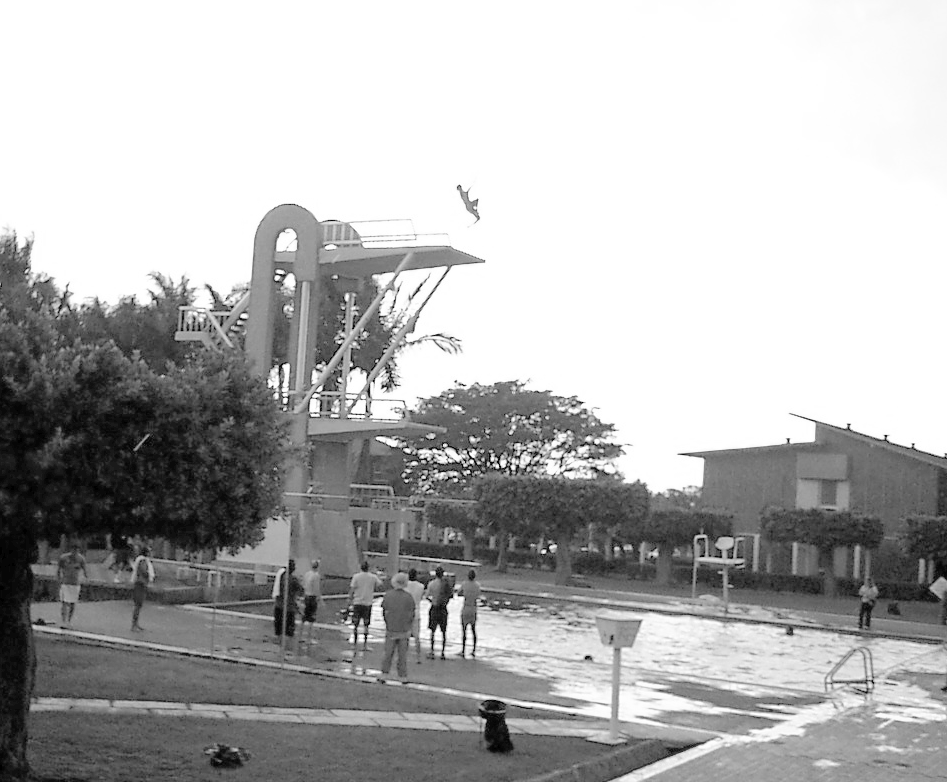
\includegraphics[width=0.9\hsize]{image200606/jumping.png}
\end{minipage}
\begin{minipage}{0.5\hsize}
今回の Debian Conference の会場は Mexico City から車で2時間ほど走ったと
ころにある Oaxtepec というリゾート地です。オリンピックに使われた会場をそ
のままリゾートホテルにしているような雰囲気です。Centro Vacacional IMSS
Oaxtepec という会場でした。プールと10mのとびこみ台などが完備されており、
ハック以外にもいろいろとできる感じがしていました。

\end{minipage}

\subsection{会の規模}

会議室は150人程度入れる会議室が準備されていました。 Hacklab として、二つの部屋
があり、それぞれには50人づつくらいが入れるようになっていたようです。

今回の参加者は登録記録によると 300 人だそうです。国別の表を次にまとめま
した
\footnote{\url{http://lists.debconf.org/lurker/message/20060518.203936.b6df5950.en.html}} 
。

今回のネットワークは 192.168.x.x で、23ビットでした。大体500台位接続でき
る計算になりますが、全員接続していた時間帯において DHCP サーバから IP が
とれなくなっていました。これは DHCP のプールを使い切っていたのではないでしょ
うか?ネットワーク自体は近くのネットカフェから無線 LAN で引っ張っていま
した。さらにこの無線 LAN をハックラボとセッションをするための会議室(通
称:タワー)を LAN でつなぐために屋根づたいで有線を引っ張っていました。

セッションも多数ありました。全体として、
参加した人数の概要も表にまとめました。

\begin{minipage}[t]{0.3\hsize}
 {\scriptsize
\begin{center}
 \begin{tabular}[t]{@{\vrule width 1pt}c|r@{\ \vrule width 1pt}}
\hline
国 & 人数 \\
\hline
 MEXICO & 144 \\
 UNITED STATES & 48 \\
 VENEZUELA & 31 \\
 GERMANY & 29 \\
 UNITED KINGDOM & 17 \\
 ITALY & 17 \\
 SPAIN & 16 \\
 EL SALVADOR & 16 \\
 BRAZIL & 16 \\
 FINLAND & 15 \\
 FRANCE & 9 \\
 COLOMBIA & 8 \\
 ARGENTINA & 8 \\
 NORWAY & 6 \\
 JAPAN & 5 \\
 CANADA & 5 \\
 BELGIUM & 5 \\
 PERU & 4 \\
 BELIZE & 4 \\
 SWITZERLAND & 3 \\
 SWEDEN & 3 \\
 NETHERLANDS & 3 \\
 INDIA & 3 \\
 GREECE & 3 \\
 CAMEROON & 3 \\
 AUSTRIA & 3 \\
 AUSTRALIA & 3 \\
 RUSSIAN FEDERATION & 2 \\
 ROMANIA & 2 \\
 NIGERIA & 2 \\
 BOSNIA AND HERZEGOVINA & 2 \\
 BOLIVIA & 2 \\
 UKRAINE & 1 \\
 NEW ZEALAND & 1 \\
 LATVIA & 1 \\
 KENYA & 1 \\
 ISRAEL & 1 \\
 IRELAND & 1 \\
 INDONESIA & 1 \\
 GUINEA & 1 \\
 GUATEMALA & 1 \\
 GAMBIA & 1 \\
 EGYPT & 1 \\
 CZECH REPUBLIC & 1 \\
 CUBA & 1 \\
 CROATIA & 1 \\
 CHINA & 1 \\
 CHILE & 1 \\
 CAMBODIA & 1 \\
 BANGLADESH & 1 \\
\hline
 \end{tabular}
\end{center} 
}
\end{minipage}
\begin{minipage}[t]{0.7\hsize}
 \begin{center}
 {\scriptsize
 \begin{tabular}{|l|l|p{20em}|r|}
\hline
日 & 時間 & タイトル & 参加人数 \\
\hline
 2006-05-14 Sunday & 11:00-11:45 & Welcome by DebConf Organizers &  50 \\
 2006-05-14 Sunday & 12:50-13:35 & wiki.debian.org BoF by Joey Hess &  29 \\
 2006-05-14 Sunday & 12:50-13:35 & OpenSolaris, Java dn Debian:  can we be friends? Simon Phipps, Alvaro Lopez Ortega &  92 \\
 2006-05-14 Sunday & 15:20-16:05 & Advanced tools for wasting time by Enrico Zini &  90 \\
 2006-05-14 Sunday & 18:00-19:00 & Multithreading:  Why and how we should use it by Ben Huthcings &  30 \\
 2006-05-15 Monday & 10:05-11:45 & Python BoF by Andreas Barth et al &  28 \\
 2006-05-15 Monday & 10:05-10:50 & Embedding Debian by Wookey &  31 \\
 2006-05-15 Monday & 11:00-11:45 & Topper: An Open Source Driver Framework by Maxim Alt and Dario Rapisardi &  59 \\
 2006-05-15 Monday & 11:55-12:40 & Ubuntu annual report by Mark Shuttleworth &  122 \\
 2006-05-15 Monday & 12:50-13:35 & i18n Infrastructure AdHoc Session I by Christian Perrier &  ~35 \\
 2006-05-15 Monday & 15:20-16:05 & Representing Debian - Doing the best for the best? by Alexander Schmehl &  ~35 \\
 2006-05-15 Monday & 16:15-17:55 & Security Enhanced Linux UML instances - an Introcution and recipe by Manoj Srivastava &  ~100 \\
 2006-05-15 Monday & 18:00-19:00 & Resurecting Computers with Free Software by Vagrant Cascadian and Hector Colina &  30 \\
 2006-05-15 Monday & 19:00-20:00 & debian-installer and SELinux by Manoj Srivastava &  ~25 \\
 2006-05-15 Monday & 21:30-22:30 & debian-installer BoF by Joey Hess &  38 \\
 2006-05-16 Tuesday & 10:05-10:50 & stable release BoF by Andreas Barth &  21 \\
 2006-05-16 Tuesday & 10:05-10:50 & ideas for repository of meta-information (watchfiles et al) by Filippo Giunchedi &  35 \\
 2006-05-16 Tuesday & 11:00-11:45 & Common Lisp development in Debian by Peter van Eynde &  8 \\
 2006-05-16 Tuesday & 11:00-11:45 & Optimizing boot time by Margarita Manterola &  100 \\
 2006-05-16 Tuesday & 11:55-13:35 & GPLv3 by Don Armstrong &  120 \\
 2006-05-16 Tuesday & 15:20-16:05 & Debian Community Guidelines by Enrico Zini &  120 \\
 2006-05-16 Tuesday & 16:15-17:55 & Let's port together. Debian fun for everyone by Peter de Schrijver and Steve Langasek &  110 \\
 2006-05-16 Tuesday & 18:00-19:00 & BoF Debian en Latinoamerica by Anibal Monsalve Salazar and David Moreno Garza &  37 \\
 2006-05-16 Tuesday & 19:00-20:00 & Scratchbox 2, bringing crosscompiling to Debian by Riku Voipio &  12 \\
 2006-05-16 Tuesday & 21:30-22:30 & Webapps Common: Tthe central point in developing a next-generation web server and web application policy by Neil McGovern &  21 \\
 2006-05-18 Thursday & 10:05-10:50 & Debian and the \$ 100 Laptop by Jim Gettys &  28 \\
 2006-05-18 Thursday & 10:05-10:50 & Governance of the Debian Project by Bdale Garbee &  57 \\
 2006-05-18 Thursday & 11:00-11:45 & X.org status and plans by Keith packard &  95 \\
 2006-05-18 Thursday & 11:55-13:35 & releasing in time - etch in December 06 by Andreas Barth and Steve Langasek &  98 \\
 2006-05-18 Thursday & 15:20-17:00 & Debian installer internals by Frans Pop &  ~~60?? \\
 2006-05-18 Thursday & 17:10-18:50 & Weeding out security bugs by Javier Fernandez-Sanguino &  47 \\
 2006-05-19 Friday & 10:05-10:50 & i18n Infrastructure AdHoc Session II by Christian Perrier &  ~30 \\
 2006-05-19 Friday & 10:05-10:50 & AM BoF &  30 \\
 2006-05-19 Friday & 11:00-11:45 & The X Community - History and Directions by Keith Packard &  70 \\
 2006-05-19 Friday & 11:55-12:40 & Experiences with large CDD-installations by Knut Yrvin &  ~100 \\
 2006-05-19 Friday & 12:50-13:35 & LTSP Muekow Next Generation by Vagrant Cascadian and Octavio H. Ruiz Cervera &  ? \\
 2006-05-19 Friday & 12:50-13:35 & the future of the NM process by Christoph Berg &  ~75 \\
 2006-05-19 Friday & 15:20-16:05 & Packaging shared libraries by Josselin Mouette &  ~50 \\
 2006-05-19 Friday & 16:15-17:55 & Cheap Thrills - Instant inspiration for the masses by Meike Reichle &  55 \\
 2006-05-19 Friday & 21:30-22:30 & What's new and cool with MySQL by Jorge del Conde &  ? \\
 2006-05-20 Saturday & 10:05-10:50 & Ubuntu Question and Answer Bof by Mark Shuttleworth &  ? \\
 2006-05-20 Saturday & 10:05-10:50 & Alternative developer's interface to APT: libapt-front by Petr Rockai &  ? \\
 2006-05-20 Saturday & 11:00-11:45 & Codes of Value: An Anthropological Analysis of Hacker Values by Gabriella Coleman &  ? \\
 2006-05-20 Saturday & 11:55-12:40 & Lightning Talks by Joey Hess et al &  ? \\
 2006-05-20 Saturday & 12:50-13:35 & www.debian.org redesign by Agnieszka Czajkowska &  ? \\
 2006-05-20 Saturday & 12:50-13:35 & Debian's Debugging Debacle: the Debrief by Erinn Clark and Anthony Towns &  ? \\
 2006-05-20 Saturday & 15:20-16:05 & debconf[67] by Andreas Schuldei &  80 \\
 2006-05-20 Saturday & 16:15-17:55 & state of the art for Debian i18n/l10n by Christian Perrier and Javier Fernandez-Sanguino &  50 \\
 2006-05-20 Saturday & 19:00-20:00 & Devotee and the temple of Doom by Manoj Srivastava &  ? \\
 2006-05-20 Saturday & 21:30-22:30 & zeroconf BoF by Joey Hess &  ? \\
\hline
 \end{tabular}
 }
 \end{center}
\end{minipage}

\clearpage

\subsection{セッション}

Debconf においてのセッションは二種類ありました。 'Talk' セッションは 90
分あり、 'BOF' セッションは45分でした。会場は Tower と Hacklab にわかれ
ていました。今回の会場は不便で、 Hacklab からTower まで歩いて20分くらい
かかりました。

\subsubsection{Topper - The Expert System ; Device Readiness Framework in Tower}

この企画は、ユーザが条件(機器データ、カーネル、ソフトウェア)データを
wikipedia のように持ちよって共有するというものです。ハードウェア互換性情
報(HCL:Hardware Compatbility List)などからアイディアをもらうというか、利
用していくのがよさそうです。

\subsubsection{Ubuntu Annual Report}

Mark Shuttleworth が Ubuntu, Kubuntu, Edu-ubuntuのこと、これからの計画の
 ことなどを Debian コミュニティ向けに説明していました。

\subsubsection{Governance of the Debian Project BOF by Bdale Garbee }

Debian Projectの歴史を振り返りつつ、DFSGやBTS, Policy Manualについて言及
し、Debian Projectの構成について説明しました。その後、問題点についてディスカッショ
ンしました。

\subsubsection{X.org status and plans BOF by  Keith Packard}

Keith Packardによる、X.orgの現状と予定についての説明です。Keith Packard 
はXにすごく入れ込んでいる人で、彼のページをみると、Xに対してすごく貢献し
ていることがわかります。内容は Xの開発方法でした。 コミュニケーションに
はemail と IRCも活用をしているようです。鍵となるプロジェクトは X Server、 
AIGLX、 Xgl、 Xlib/XCB など Desktop 関係でXに興味があるなら気になるキー
ワードがいっぱいありました。

Xは、モノリシックな構造からモジュール化の構造へ移行するべく作業中である
とのことです。Debian は、X.org 7.x系に移行しました。 Keith Packard が、
X.orgのi810 driverをハックしたときの事を話してくれました。

X.org のソース管理リポジトリーは、これまで cvs だったけど、 Keith
Packard がgitに変えたとのことです。

\subsubsection{The X Community - History and Directions by Keith Packard}

Keith Packard による X のセッション。彼曰く、X Consortium はひどかった。
The Open Groupに移管された後、XFree86 が実質的な権限をもっていたそうです。
XFree86 は X Consortium に参加するため企業として登録されていたのですが、
登録を簡単にするために必要最低限の会則だけを最初につくったそうです。この
時点では実際は一人で運営されており、最終的に開発者が追放されたり、ライセ
ンスが変更になったりしました。

Xorgになってよかったね、という結論でした。

このプロジェクトの教訓としては

\begin{itemize}
 \item ガバナンス重要
 \item いそいでつくりあげてしまったものは長い間残ってしまう
 \item いろいろと参加して、オープンで居続けるべき
\end{itemize}

ということだそうです。

\subsubsection{releasing in time - etch in December 06 by Andi Barth and Steve Langasek }


Etchのリリースについて、testingへパッケージが入る方法を説明して、Etchに
残っている問題を列挙しました。 toolchain、 X.org、 docs-in-main、
firmware-in-main、mirror-split AMD64、 secure aptなどの問題があるも大体
メドはついたとのことです。gcc 4.1, python2.4も問題です。QAは自動的にパッ
ケージをインストールする方法について話しがあった模様です。また brinteyへ
のヒント, 疑似パッケージをリリースノートへ, リリースをするときには、コー
ドネームを使う, ベースのフリーズを短く、細かく, binNMUをもっと活用する、
などの提案がありました。
Andreas Barth(aba)の英語は聞きづらくて、よくわかりませんでした。

各アーキテクチャの状態は architecture re-qualification status for etch
\footnote{\url{http://release.debian.org/etch_arch_qualify.html}}, 自分
のメンテナンスしているパッケージ状態は Package status
\footnote{\url{http://people.debian.org/~igloo/status.php}}で確認するこ
とができます。

\subsubsection{Debian Installer internals by Frans Pop }

GUIベースの新しいインストーラをみせて、参加者から拍手があがりました。VMwareをつかっ
てD-Iの説明。D-IのDebug方法。CDD(Custom Debian Distributions)の話題が出
ました。

udebのことと、D-I(Debian Installer)のことについて説明していました。
Debian installer に足りない機能とはなにか?という話しで、ライセンスキー
の入力!というジョークを飛ばして会場の笑いを取っていました。実際にライセ
ンスキー入力モジュールを作成し、udebの作成方法、Debian InstallerのCD
image作成について例をみせながらやってくれました。

\subsubsection{AM(Application Manager) Meeting}

AMは、担当者によって対応が異なるという点などをディスカッションしました。
議論が白熱して別のセッションが行われる事になりました。矢吹はこのセッショ
ンには、自分のAMに会いにいくためだけに参加しました。

\subsubsection{The Future of the NM Process}

新しいDebian Developerになるための要件やプロセスについてディスカッション
しました。

Proposal, Credit: Anthony Towns, Mike Brockschmidt, Get input
feedback ということで、まず現在の状況をまとめていました。そして現在の問
題点の整理をしました。新しいプロセスは、
ITP、Package作成、スポンサードアップロードをしたことがあるかどうかという
ことを確認することになるようです。
Debianへの貢献(バグ修正やnew upstreamパッケージ作成など)をどれくらいして
いるのか、も尺度になるようです。

\subsubsection{Debian's Debugging Debacle by Erinn Clark and Anthony Towns }

 一般的なデバッグ手法についてから、Debian固有のデバッグ方法についてのトー
 クでした。

まず、printfデバッグの良い点は簡単、まずいところはプログラムの実行が遅く
なるということを説明していました。その後、 straceデバッグの良い点として
OSとプログラムのやりとりがよくわかるという点をあげていました。また、ソー
スコードなどにアクセスしなくてもよいということをあげました。Symbolic デ
バッグについてのDebianでのアプローチは、デバッグを簡単にするよりもバイナ
リーのサイズを小さくするためにデバッグシンボルをつける付けないは環境変数
を設定して再ビルドするという現状を紹介しました。ELF の DWARF 構造をなん
とかして処理したいという話しで、elfutils のdebugedit が便利なのだが、フ
リーではない、どうしたらよいんだ!という話しの展開でした。デバッグにはバ
イナリパッケージとソースパッケージが両方必要で、デバッグ情報からソースコー
ドへのリンクをどうするべきなのか、ということを検討していました。

会場からelfutilsがフリーになってリリースされたとの情報がでて、場内から拍
手が起きていました。

\subsubsection{Embedded Debian BOF by wookey}

PowerPC/ARM/SuperHについて語っていました。 dpkg-cross / cross compile に
ついて、どのようにしているのかを話しました。SHも対象ターゲットに入ってい
るということ。SH4はやってないようですが、SH3を使って行っているようです

\subsubsection{100 dollar PC by Jim Gettys}

ハードウェアを開発しており、もうすこしで、サンプルボードが出荷されるそう
です。ただ、消費電力を少なくするために、白黒の液晶を反射型ではなく透過型
を利用するらしく、まだ生産できていないようです。子どもは5W-10W程度の電力
を発電できるそうで、それで駆動させるために、1W程度の消費電力におさえてい
るそうです。

ソフトウェアの革命的な変更が必要だ、と主張していました。

CPUはGeodeだそうです。

本来はキーを押すたびにスリープから復活するような設計にするつもりだったの
ですが、そうすると100ms程度かかってしまうので、反応が悪すぎてあきらめたそうです。


\subsubsection{GPL v3}

GPL v3 についての議論をしました。

DebianとしてGPL v3 の策定に参加しているので、意見があるのなら、コーディ
ネータにメールするようにという事です。

次のドラフトがもうすぐでるので、それに対してまたコメントしましょう、とい
うことでした。

\subsubsection{Debian Community Guidelines}

Enrico Zini によるDebian Community Guidlines。Debian 内のコミュニティに
関するガイドラインのお話。完璧なものや、ポリシーではなく、効率よく活動で
きるためにはどうしたらいいのか、というガイドライン。コードを読みながら、
話し合おうとか、バグを正確に取って、Upstream に還元しましょうなどなどの
話題でした。

\subsubsection{Let's port together. Debian fun for everyone}

Debian を新しいアーキテクチャにポーティングする際の注意点などについて議
論しました。エンディアン、C言語の注意点、アライメントについてや、CPU , 
周辺機器についての話題がありました。いっしょにポーティングしましょう、と
いうことが言いたかったようです。

\subsubsection{Packaging shared libraries by Josselin Mouette}

Josselin Mouette(joss) が shared libraryのパッケージングについて話しまし
た。みんなは本当に、ちゃんとshared libraryのパッケージ方法、メンテナンス
方法知っているのか?こうやってやるんですよ、と話してくれました。

例えば、ライブラリでABI の変更があった場合、そのパッケージに依存するパッ
ケージは再ビルドが必要で、shlibs ファイルを適正に生成するために 
\verb!dh_makeshlibs -V'hogehoge (>=0.0.1)'! 等を行う必要があります。ま
た、リリースするタイミングはライブラリのメンテナ次第なので、手助けしましょ
うと言ってました。

彼はアニメ好きのようで、壁紙が舞-乙HiMEでした。Joss と話すと、舞-乙HiMEがお気に入りという
ことがわかりました。

\subsubsection{Codes of Value: An Anthropological Analysis of Hacker Values by Gabriella Coleman}

Biella Colemanが自分の社会学の研究成果について説明していました。Debian 
を研究してドクターをとったそうです。

\subsubsection{translation/i18n BOF}

3回に及ぶBOFでした。
翻訳についての現状とこれからについて議論していました。

初回は、ロゼッタのことで盛り上がりました。Rosetta などの既存の新しいツー
ルでは解決できない問題、これからどうしていきたいのか、と言う事について話
し合われました。

\subsubsection{Lightning Talk}
\begin{itemize}
	\item Actively Discovering bugs/issues with packages
	\item Walkthrough : Make your Country love Debian
	\item Debian in the greater Linux ecosystem
	\item WNPP: Automatizing the unautomatizable
	\item How far can we go with a collaborative maintenance infrastructure
	\item How to get debian-admin to help you
	\item Learning from Gentoo
	\item Datamining on Debian packages metadata
	\item Tracking MIA developers
	\item How to pronounce Jeroen van Wolffelaar, and other names
\end{itemize}

	ライトニングトーク。Gentooを見習って、ドキュメントとか整備しろ!
	とか、上川 純一という名前は言いにくいなどの話題が出ました。

\subsubsection{debconf67 BOF}

結論が出ませんでした。

各サイトの担当者が発表し、情報を比較しました。イギリスとボズニアが候補の
ようです。

\subsection{キーサインパーティ}
 Debconf の醍醐味のひとつである、Key Sign party を行いました。
今回は140人ほど集まり、2時間かけてせっせとKey Sign しました。

矢吹さんがチェックサムを間違えて\footnote{最新のキー一覧を取得
して計算してなかったのが敗因です。コーディネータが数字を読み上げた時に、
かなり焦りましたが、もう一度取得しなおして再計算したら合ったので入れても
らいました by yabuki}、半分ぐらいの人しか Key Sign できなかったのはここだけの秘密
です。

\subsection{参考文献}

参考になる過去の文献を列挙します。

\begin{itemize}
 \item 後藤さん、2005年の報告: \url{http://gotom.jp/~gotom/pub/Debconf5/}
 \item 後藤さん、2004年の報告: \url{http://www.gotom.jp/~gotom/linux/Debconf4/}
 \item 鵜飼さん、2003年の報告: \url{http://ukai.jp/Slides/2003/0725-fsij/}
 \item 上川等、2006年に検討しているDebconf日本開催Wikiページ \url{http://wiki.debian.org/DebConfInJapan}
 \item 武藤さん等、2005年に検討したDebconf日本開催Wikiページ \url{http://kmuto.jp/open.cgi?debconf-in-japan}
\end{itemize}

\dancersection{pbuilder cowdancer cowbuilder}{上川}

\texttt{cowbuilder} は Debian の QA のためのツールです。今回Debconfの会
場で開発しました。基本となるメカニズムである \texttt{cowdancer} 自体は 
Finland での Debconf (2005年) で開発を開始しましたが、当時から構想をねっ
ていた \texttt{cowbuilder} に着手し完了したのは、 Mexico での Debconf
(2006年) でした。

本論文では Debian の QA 用のツールである \texttt{pbuilder} とファイルシ
ステムをcopy-on-write 的に利用するためのツールである \texttt{cowdancer} 
の説明をして、その後その二つを組み合わせたアプリケーションである 
\texttt{cowbuilder} の説明をします。

\subsection{pbuilderとは}

まず、\texttt{cowbuilder} のベースになっている \texttt{pbuilder} につい
て紹介します。

\texttt{pbuilder}\footnote{\url{http://pbuilder.alioth.debian.org/},
\url{http://www.netfort.gr.jp/~dancer/software/pbuilder.html.ja}} は 
Debian パッケージのビルドテストをクリーンルーム環境({\tt chroot})で実施
することが簡単になるようにつくられたツールです。{\tt chroot}環境を利用す
ると、いろいろな試験を実施することができますが、実はバージョンを最新にす
る手間とか、最小のパッケージをインストールするための手間などが結構かかり
ます。特に、いつでも最新版の \texttt{Debian} をインストールできる必要が
あるため、ときおりトラブルが起き、その問題を解決する必要があります。そこ
で、 \texttt{chroot} 管理に関連した QA 作業を集中してスクリプト化してお
き、このスクリプトさえ使えばいつでも動くようにしてしまおう、という目論見
ではじめたのが \texttt{pbuilder} です。

ここで解説している対象はバージョン 0.155 です。

{\tt pbuilder build {\it パッケージ.dscファイル} }コマンドを利用すると、
tar.gz から \texttt{chroot} を展開して、その中でDebian パッケージをビル
ドしてくれます。ビルドに必要な依存関係は \texttt{debian/control} ファイ
ルの \texttt{Build-Depends} フィールドと \texttt{Build-Depends-Indep} 
フィールドを参考に \texttt{apt-get install} でインストールしてくれます。

{\tt pbuilder create} は Debian の初期インストールイメージを作成し、 
tar.gz として管理します。\texttt{--basetgz} オプションを利用すれば、
tar.gzファイルを指定できます\footnote{デフォルトは 
\texttt{/var/cache/pbuilder/base.tgz}}。\texttt{--distribution}オプショ
ンでディストリビューション(etch/sarge/sid) を指定することができるので、
各バージョン用の\texttt{chroot} 環境を作成することができます。通常は
unstable 対象に開発作業を実施するので、 sid がデフォルトです。

{\tt pbuilder update} は Debian の初期インストールイメージを最新版の状態
に更新します。Debian unstableは一日一回新しいバージョンがリリースされて
しまうので、一日に一回実行する必要があります。

{\tt pdebuild} は、一般ユーザ権限で、カレントディレクトリが Debian パッ
ケージのソースディレクトリの中\footnote{debian/ ディレクトリがある場所}
の場合に、 sudo コマンドを利用して root 権限に昇格し、Debianのソースパッ
ケージの作成から \texttt{chroot} 環境でのパッケージビルドまでの一連の動
作を自動化してくれます。

ここから、\texttt{pbuilder create}, \texttt{pbuilder update},
\texttt{pbuilder build}, \texttt{pdebuild} のそれぞれの実行時のログの例
を紹介します。

\begin{commandline}
# pbuilder update --mirror http://ftp.jp.debian.org/debian --override-config --distribution sid 
W: /home/dancer/.pbuilderrc does not exist
Upgrading for distribution sid
Building the build Environment
 -> extracting base tarball [/var/cache/pbuilder/base.tgz]
 -> creating local configuration
 -> copying local configuration
 -> mounting /proc filesystem
 -> mounting /dev/pts filesystem
 -> policy-rc.d already exists
  -> Installing apt-lines
Refreshing the base.tgz 
 -> upgrading packages
Get:1 http://ftp.jp.debian.org sid Release.gpg [189B]
Get:2 http://ftp.jp.debian.org sid Release [38.3kB]
Ign http://ftp.jp.debian.org sid Release
Get:3 http://ftp.jp.debian.org sid/main Packages [4030kB]
Fetched 4069kB in 4s (904kB/s)
Reading package lists... Done
W: GPG error: http://ftp.jp.debian.org sid Release: Could not execute '/usr/bin/gpgv' to verify signature 
 (is gnupg installed?)
W: You may want to run apt-get update to correct these problems
dpkg - warning: ignoring request to remove lilo which isn't installed.
Obtaining the cached apt archive contents
Reading package lists... Done
Building dependency tree... Done
Calculating upgrade... Done
The following NEW packages will be installed:
  cpp-4.1 g++-4.1 gcc-4.1 libstdc++6-4.1-dev tasksel-data
The following packages will be upgraded:
  apt apt-utils aptitude bsdutils coreutils cpio cpp cpp-4.0 debconf
[中略]
  wget
77 upgraded, 5 newly installed, 0 to remove and 0 not upgraded.
Need to get 25.4MB/49.3MB of archives.
After unpacking 25.4MB of additional disk space will be used.
WARNING: The following packages cannot be authenticated!
  bsdutils dpkg coreutils debianutils diff libc6-dev tzdata libc6 e2fslibs
[中略]
  libgnutls12 telnet dhcp3-client dhcp3-common
Get:1 http://ftp.jp.debian.org sid/main dpkg 1.13.21 [1569kB]
[中略]
Get:41 http://ftp.jp.debian.org sid/main telnet 0.17-32 [72.1kB]
Fetched 25.4MB in 17s (1423kB/s)
Extracting templates from packages: 100%
Preconfiguring packages ...
(Reading database ... 12009 files and directories currently installed.)
Preparing to replace bsdutils 1:2.12r-9 (using .../bsdutils_1%3a2.12r-10_amd64.deb) ...
Unpacking replacement bsdutils ...
Setting up bsdutils (2.12r-10) ...

[中略]

Preparing to replace libgpg-error0 1.2-1 (using .../libgpg-error0_1.2-1_amd64.deb) ...
Unpacking replacement libgpg-error0 ...

[中略]

Setting up libc6-dev (2.3.6-15) ...

[中略]

Setting up dpkg-dev (1.13.21) ...
Reading package lists... Done
Building dependency tree... Done
build-essential is already the newest version.
dpkg-dev is already the newest version.
apt is already the newest version.
0 upgraded, 0 newly installed, 0 to remove and 1 not upgraded.
Copying back the cached apt archive contents

[中略]

 -> new cache content libgnutls12_1.2.11-1_amd64.deb added
 -> unmounting dev/pts filesystem
 -> unmounting proc filesystem
 -> creating base tarball [/var/cache/pbuilder/base.tgz]
 -> cleaning the build env 
    -> removing directory /var/cache/pbuilder/build//2252 and its subdirectories
\end{commandline}

\begin{commandline}
$ sudo pbuilder build ~/pending/20060531/pbuilder_0.154.dsc 
W: /home/dancer/.pbuilderrc does not exist
I: using fakeroot in build.
pbuilder-buildpackage/amd64 Id: xxxx
Id: xxxx

Current time: Sat Jun 10 23:42:44 JST 2006
pbuilder-time-stamp: 1149950564
Building the build Environment
 -> extracting base tarball [/var/cache/pbuilder/base.tgz]
 -> creating local configuration
 -> copying local configuration
 -> mounting /proc filesystem
 -> mounting /dev/pts filesystem
 -> policy-rc.d already exists
 -> created buildresult dir :/var/cache/pbuilder/result/
Obtaining the cached apt archive contents
Installing the build-deps
 -> Attempting to parse the build-deps : pbuilder-satisfydepends,v 1.28 2006/05/30 23:45:45 dancer Exp $
 -> Considering  debhelper (>= 4.1.0)
   -> Trying debhelper

[中略]

 -> Installing  debhelper docbook-xsl ldp-docbook-xsl xsltproc
Reading package lists... Done
Building dependency tree... Done
The following extra packages will be installed:

[中略]

0 upgraded, 14 newly installed, 0 to remove and 1 not upgraded.
Need to get 2643kB/5118kB of archives.
After unpacking 23.1MB of additional disk space will be used.
WARNING: The following packages cannot be authenticated!
  libmagic1 file html2text gettext intltool-debian po-debconf debhelper
  sgml-base xml-core docbook-xsl ldp-docbook-xsl libxml2 libxslt1.1 xsltproc
Get:1 http://ftp.jp.debian.org sid/main libmagic1 4.17-1 [277kB]

[中略]

Get:10 http://ftp.jp.debian.org sid/main xsltproc 1.1.17-1 [100kB]
Fetched 2643kB in 2s (953kB/s)
Selecting previously deselected package libmagic1.
(Reading database ... 12605 files and directories currently installed.)
Unpacking libmagic1 (from .../libmagic1_4.17-1_amd64.deb) ...
Selecting previously deselected package file.

[中略]

Setting up xsltproc (1.1.17-1) ...
 -> Finished parsing the build-deps
Reading package lists... Done
Building dependency tree... Done
The following NEW packages will be installed:
  fakeroot

[中略]

Copying source file
    -> copying [/home/dancer/pending/20060531/pbuilder_0.154.dsc]
    -> copying [/home/dancer/pending/20060531/pbuilder_0.154.tar.gz]
Extracting source
su: Authentication service cannot retrieve authentication info.
(Ignored)
dpkg-source: warning: no utmp entry available and LOGNAME not defined; using uid of process (1234)
dpkg-source: warning: could not verify signature on ./pbuilder_0.154.dsc since gpg isn't installed
dpkg-source: extracting pbuilder in pbuilder-0.154
dpkg-source: unpacking pbuilder_0.154.tar.gz
 -> Building the package
su: Authentication service cannot retrieve authentication info.
(Ignored)
dpkg-parsechangelog: warning: no utmp entry available and LOGNAME not defined; using uid of process (1234)
debian: warning: no utmp entry available and LOGNAME not defined; using uid of process (1234)

[中略]

 fakeroot debian/rules clean

[中略]

 debian/rules build

[中略]

 -> unmounting dev/pts filesystem
 -> unmounting proc filesystem
Current time: Sat Jun 10 23:43:47 JST 2006
pbuilder-time-stamp: 1149950627
 -> cleaning the build env 
    -> removing directory /var/cache/pbuilder/build//10498 and its subdirectories

\end{commandline}

\begin{commandline}
$ pdebuild 
W: /home/dancer/.pbuilderrc does not exist
dpkg-buildpackage: source package is pbuilder
dpkg-buildpackage: source version is 0.155
dpkg-buildpackage: source changed by Junichi Uekawa <dancer@debian.org>
dpkg-buildpackage: source version without epoch 0.155
 fakeroot debian/rules clean
dh_testdir
dh_testroot
rm -f build-stamp configure-stamp
# Add here commands to clean up after the build process.
/usr/bin/make clean
make[1]: Entering directory `/home/dancer/cvscheckout/external/pbuilder/pbuilder'
rm -f *.bak *~ TAGS
rm -f testsuite/testimage
rm -rf testsuite/testbuild testsuite/testbuild2
make[1]: Leaving directory `/home/dancer/cvscheckout/external/pbuilder/pbuilder'
rm -rf debian/pbuilder-uml/
dh_clean
 dpkg-source -b pbuilder
dpkg-source: warning: source directory `./pbuilder' is not <sourcepackage>-<upstreamversion> `pbuilder-0.155'
dpkg-source: building pbuilder in pbuilder_0.155.tar.gz
dpkg-source: building pbuilder in pbuilder_0.155.dsc
 dpkg-genchanges -S
dpkg-genchanges: including full source code in upload
dpkg-buildpackage: source only upload: Debian-native package
W: /home/dancer/.pbuilderrc does not exist
I: using fakeroot in build.
pbuilder-buildpackage/amd64 Id: xxxx
Id: xxxx

Current time: Sat Jun 10 23:49:35 JST 2006
pbuilder-time-stamp: 1149950975
Building the build Environment
 -> extracting base tarball [/var/cache/pbuilder/base.tgz]
 -> creating local configuration
 -> copying local configuration
 -> mounting /proc filesystem
 -> mounting /dev/pts filesystem
 -> policy-rc.d already exists
 -> created buildresult dir :/var/cache/pbuilder/result
Obtaining the cached apt archive contents
Installing the build-deps

[中略]

dpkg-buildpackage: full upload; Debian-native package (full source is included)
Copying back the cached apt archive contents
 -> unmounting dev/pts filesystem
 -> unmounting proc filesystem
Current time: Sat Jun 10 23:50:38 JST 2006
pbuilder-time-stamp: 1149951038
 -> cleaning the build env 
    -> removing directory /var/cache/pbuilder/build//13247 and its subdirectories
\end{commandline}


\subsection{cowdancerとは}

\texttt{cowdancer}\footnote{\url{http://www.netfort.gr.jp/~dancer/software/cowdancer.html.ja}} 
はディレクトリをハードリンクでコピーしておけば、ファイルに書き込みが発生
する段階でハードリンクの関係を破壊してくれる、というツールです。大きなディ
レクトリツリーを作業用にコピーして、作業したあとは捨てる、と言うような利
用方法の場合、実際にコピーすると書き込み量が大きく、待たされます。また全
てのファイルを変更するわけではなく、一部のファイルしか書き換えないので、
書き換える段階になってから実物をコピーしたほうが効率良い場合があります。
そのような用途に利用します。

GNU の \texttt{cp} コマンドであれば、 \texttt{cp -al} でコピーをすると、
ファイルを全部コピーするかわりに全てのファイルをハードリンクでコピーして
くれます。\texttt{cp -al} でコピーしたツリーに対して、 
\texttt{cow-shell} コマンドで起動したシェルの中で作業すればよいです。

例えば、下記のような作業をしても、\texttt{linux-2.6} ディレクトリの中身
には影響を与えません。また、\texttt{cp -a} コマンドでコピーするのに比べ
ると格段に速いです。

\begin{commandline}
$ cp -al linux-2.6 linux-2.6-work
$ cd linux-2.6-work
$ cow-shell 
Invoking /bin/bash
$ vi .config
[作業]
$ exit 
exit
$ cd ../
$ rm -rf linux-2.6-work
\end{commandline}

\subsection{cowbuilderとは}

\texttt{cowbuilder} は \texttt{cowdancer} を利用して \texttt{pbuilder} 
を高速化したツールです。\texttt{pbuilder} は便利ですが、Debian のインス
トールイメージの .tar.gz を毎回展開しているため、遅いという重大な欠点が
ありました。.tar.gz のかわりに作業用のツリーを展開した状態で保持しておき、
\texttt{cowdancer} を利用して、ハードリンクを毎回利用するようにしたとこ
ろ、.  .tar.gz の展開の部分が省略されたため、高速になりました。

\subsection{cowbuilderの使い方}

ここで解説している対象はバージョン 0.17 です。

{\tt cowbuilder --build {\it パッケージ.dscファイル} }コマンドを利用する
と、Debian パッケージを \texttt{cowbuilder} 環境の \texttt{chroot} 内部
でビルドしてくれます。ビルドに必要な依存関係は \texttt{debian/control} 
ファイルの \texttt{Build-Depends} フィールドと 
\texttt{Build-Depends-Indep} フィールドを参考に \texttt{apt-get install} 
でインストールしてくれます。

{\tt cowbuilder --create} は Debian の初期インストールディレクトリを作成
します。今後はそのディレクトリを \texttt{chroot} で活用することにな
ります。\texttt{--basepath} オプションを利用すれば、ディレクトリを配置す
る場所を指定できます。\footnote{デフォルトは
\texttt{/var/cache/pbuilder/base.cow}}。\texttt{--distribution}オプショ
ンでディストリビューション(etch/sarge/sid) を指定することができ、各バー
ジョン用の\texttt{chroot} 環境を作成することができます。通常はunstable 
対象に開発作業を実施するので、 sid がデフォルトです。

{\tt cowbuilder --update} は Debian の初期インストールイメージを最新版の
状態に更新します。 Debian unstable は一日一回新しいバージョンがリリース
されてしまうので、一日に一回実行する必要があります。

{\tt pdebuild --pbuilder cowbuilder} は、一般ユーザ権限で、カレントディ
レクトリが Debian パッケージのソースディレクトリの中\footnote{debian/ ディ
レクトリがある場所}の場合に、 sudo コマンドを利用して root 権限に
昇格し、Debianのソースパッケージの作成から \texttt{chroot} 環境でのパッ
ケージビルドまでの一連の動作を自動化してくれます。

\subsection{cowbuilder 実行時間計測結果}

計測してみた例(秒)を表にしてみました。計測に利用したマシンは 2006年5月時
点ころの Debian GNU/Linux sid Apple iBook G4 ppc 1GHz です。

\begin{center}
 \begin{tabular}[t]{@{\vrule width 1pt}l|r|r|r@{\ \vrule width 1pt}}
 \hline
 \hline
 オペレーション & pbuilder & cowbuilder & speed \\
 \hline
 update & 150  & 16 & 10x \\
 build (N/W down) & 80 & 18 & 5x \\
 build (pbuilder) & 177 & 86 & 2x\\
 login & 80 & 4 & 20x\\
 \hline
 \hline
 \end{tabular}
\end{center}

update は \texttt{pbuilder update} と \texttt{cowbuilder --update} の比
較です。あきらかに tar.gz を展開して再度作成するコストがなくなるので高速
になります。一日一回は実施するコマンドなので、高速化するメリットはあるで
しょう。

build (N/W down) は \texttt{pbuilder build} と \texttt{cowbuilder
--build }をネットワーク接続がない状態で実行した場合です。これは依存関係
を満たすためのパッケージの取得ができなかった場合の時間を計測しています。 
ビルド環境を作成して削除するまでの純粋な時間を計測しています。

build (pbuilder) は \texttt{pbuilder} パッケージを \texttt{pbuilder
build} と \texttt{cowbuilder --build} でそれぞれビルドした場合の例です。
パッケージのインストール処理自体が動くとその処理に時間がかかるので、差が
縮まっているのがわかります。でも二倍高速化しています。

login は \texttt{pbuilder login} と \texttt{cowbuilder --login} でそれぞ
れログインしてすぐに exit するまでの時間を計測しました。ちょっとしたコマ
ンドを試したりテスト環境を構築するのに login をすることが多いのですが、
その状況で一分待たせるのか、4秒しか待たないのか、というのでは大きな差が
出て来ます。

\subsection{cowbuilderの今後の課題}

\texttt{debuild} を利用してパッケージをビルドする時間と比較してみると、
実はまだまだ高速化できる余地はあります。\texttt{apt-get} でベースインス
トールイメージからBuild-Depends をそろえる部分にて、時間を取られているこ
ともあり、また、ext3 ファイルシステムを利用している場合、ハードリンクし
たツリーの \texttt{rm -rf} が結構遅いこともあります。今後の方策としては
いろいろありますが、たとえば下記が考えられます:

\begin{itemize}
 \item 各パッケージ向けのインストールイメージのキャッシュ。\texttt{Build-Depends} 
       の解析は一パッケージ一日一回ですむようにして、ビルドツリーのキャッ
       シュを保持しておく。
 \item \texttt{apt-get install} を高速化する, \texttt{dpkg -i} を高速化する, \texttt{dpkg} をデーモ
       ン化させ、 \texttt{apt-get} からはデーモンを呼ばせる
 \item \texttt{ext3}ファイルシステムの削除ルーチンの高速化、もしくは高速
       な削除ができるファイルシステムへの移行。
\end{itemize}

\texttt{apt-get install} の高速化は日常的な管理のオペレーションにとって
も利点があるので、そちらを注目して作業してみるとよいでしょう。

\dancersection{次回}{}

北海道で合宿を開催し、また遠隔セッションをIRCで開催する予定です。
内容は本日決定予定です。

参加者募集はまた後程。

\newpage

\vspace*{15cm}
\hrule
\vspace{2mm}

\includegraphics[width=2cm]{image200502/openlogo-nd.eps}
\noindent \Large \bf Debian 勉強会資料\\ \\
\noindent \normalfont 2006年6月17日 \hspace{5mm}  初版第1刷発行\\
\noindent \normalfont 東京エリア Debian 勉強会 (編集・印刷・発行)\\
\hrule

\end{document}

% LocalWords:  Debconf BOF SuperH Ubuntu knoppix pbuilder cowbuilder pdebuild
% LocalWords:  chroot sudo cowdancer Brockschmidt
